
\clearpage
\cleardoublepage

\chapter{Geo Spatial Data Pre-processing Pipeline}
\label{chap:preprocess}
\begin{figure}[h]
    \centering
    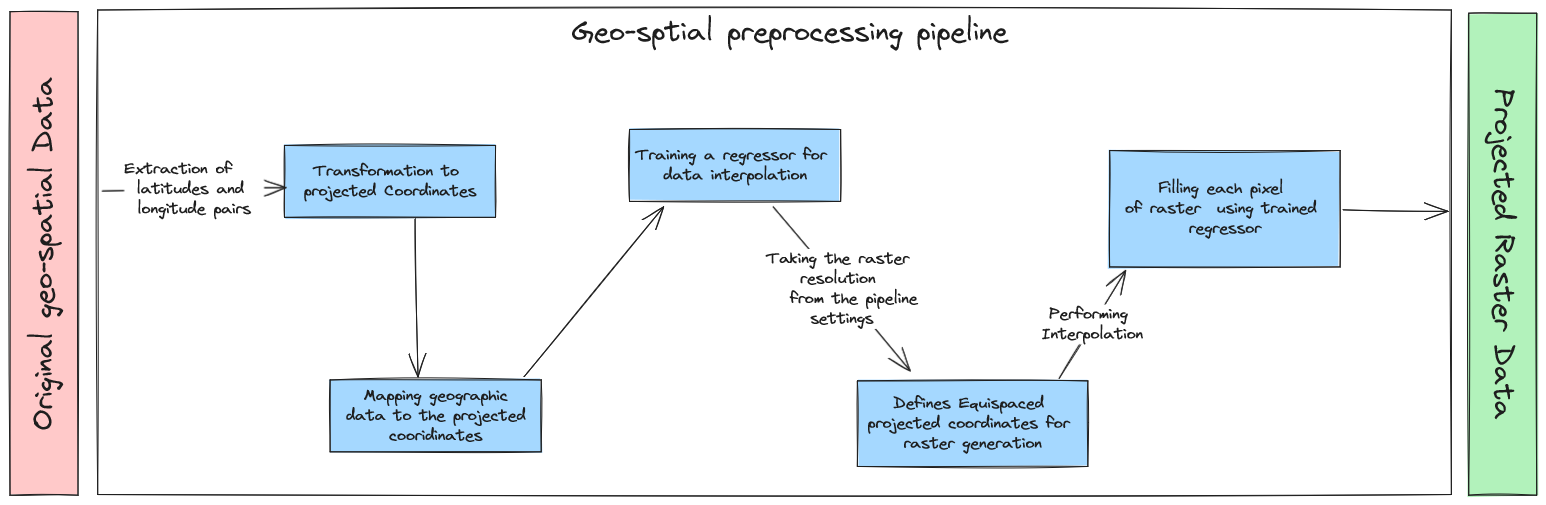
\includegraphics[width=1.0\linewidth]{figures/chapter-7/preprocessing_pipeline.png}
    \caption{geospatial preprocessing pipeline}
    \label{fig:preprocessingpipeline}
\end{figure}
The preceding sections thoroughly explain the geospatial data used to evaluate the convolutions on map projections. In geospatial analysis, the raw data, which maps geo coordinates to the data, cannot be used directly. Scientists commonly employ a preprocessing step to analyze the geospatial data. The data in use, which consists of the monthly observations of geopotential height and precipitation, needs to go through a process and be transformed into a format that could be easily analyzed.

There are two ways to transform the raw data into reduced spatial entities. These reduced spatial entities are classified as Vector or Raster data models, both acceptable by most GIS software.

As our interest is in map projections, the purpose of the preprocessing pipeline is to generate map projection rasters from the raw data. Different Python libraries are utilized for this raster generation. The initial sections of the current chapter explain these tools and libraries.

\section{Data Raster}
\begin{figure}[h]
    \centering
    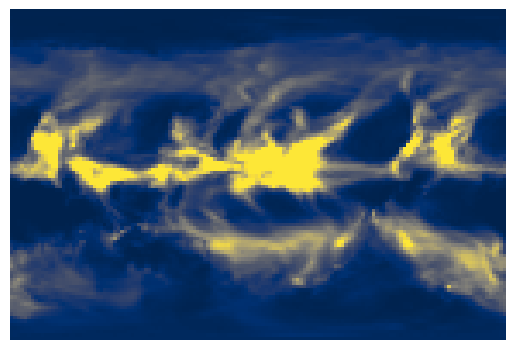
\includegraphics[width=0.75\linewidth]{figures/chapter-7/precipitation_raster_thesis.png}
    \caption{Precipitation raster data with dimensions 96x144}
    \label{fig:precipitation-raster}
\end{figure}
Raster data is employed in the analysis of geographical data. A raster is a grid structure containing data, wherein each cell signifies the data's actual value. The raster's coordinates are determined by its resolution, representing the transformed projected reference system coordinates.


\section{Proj and python's pyproj Package}


\subsection{Proj}
The primary purpose of PROJ is that it is a coordinate transformation
software. It converts the geospatial coordinates from one coordinate reference system (CRS) to another CRS. The software allows transformations to cartographic projection or projected reference systems and geodetic reference systems. The PROJ software provides a command-line interface to interact with its main functionality. The command-line interface can transform from the coordinates provided as user input or files. It also exposes an API to interact programmatically. The ease of usage to interact with the functionality of the PROJ software makes it a popular choice among the different Python libraries and packages that process geospatial data.

"Cartopy" is a popular package for geospatial data visualization. It also uses PROJ when dealing with coordinate reference system transformations. Different data visualization and processing libraries, such as matplotlib, array, and geoPandas, provide interfaces to incorporate Cartopy.

The PROJ software provides an extensive list of map projections. Though the number of map projections in the literature is too great to incorporate into the software, it still provides ample map projections. The software also provides a geodetic transformation facility.

"Reference: taken from PROJ project about page."

\subsection{Proj strings}

Before discussing the Proj strings, it is necessary to discuss the different formats used for storing the information of coordinated reference systems. Multiple formats are used for encoding a coordinate reference system. In light of this thesis, mentioning EPSG codes and WKT is deemed essential to bring discussion to the Proj4 strings.

The primary standard in use is the well-known text WKT. WKT is standardized by the Open Geospatial Consortium (OGC). This format describes the geographic features as standardized text representation. The WKT can represent vector geometry objects, spatial reference systems of spatial objects, and transformations between spatial reference systems (SRS). The significance of WKT lies in its ability to provide a concise and easily understandable representation of various geometric objects, including lines, polygons, triangulated irregular networks (TINs), polyhedrons, and enclosed areas on a map. Furthermore, it serves as a valuable tool for succinctly describing the essential components of coordinate reference system (CRS) definitions, enabling efficient communication and analysis within spatial data. The details for the standard are at \url{"https://docs.ogc.org/is/18-010r11/18-010r11.pdf"}
\begin{lstlisting}
POLYGON ((0 0, 4 0, 4 4, 0 4, 0 0), (1 1, 1 2, 2 2, 2 1, 1 1))
\end{lstlisting}
The European Petroleum Survey Group (EPSG) code is one of the other standards for encoding CRS. EPSG codes are primarily four digits long, but the number of code digits can increase. These codes are specific to only one projected reference system or coordinate systems of different types. The EPSG:4326 describes simple longitude and latitude pairs, which represent the Datum of WGS84.

The Proj.4 strings do incorporate the projected reference system well. The main advantage of using the "Proj.4" strings is that they are human-readable. It is a string that provides different parameters to control the different aspects of the geographic or projected transformation. Here is an example of a "Proj.4" string.

\begin{figure}[h]
    \centering
    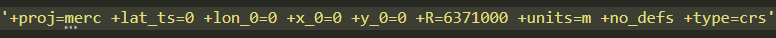
\includegraphics[width=1.0\linewidth]{figures/chapter-7/proj_string_mercator.png}
    \caption{Proj.4 string for Mercator projection}
    \label{fig:proj-string-mercator}
\end{figure}

All the arguments in the "Proj.4" format string start with a plus (+) sign. The values are assigned to the arguments using an equal sign (=), just as one will do when handling the command line arguments with longer names. The most prominent arguments of the string are +proj and +type. The +type argument tells the PROJ software which type of transformation occurs in the string. The type of transformation is between coordinate reference systems. As mentioned in the earlier sections, the projected reference system is a coordinate reference system. The argument +proj tells the name of the projection. The above "Proj.4" string argument has the value of "merc," which indicates transformation happens to  Mercator projection.
\begin{figure}[h]
    \centering
    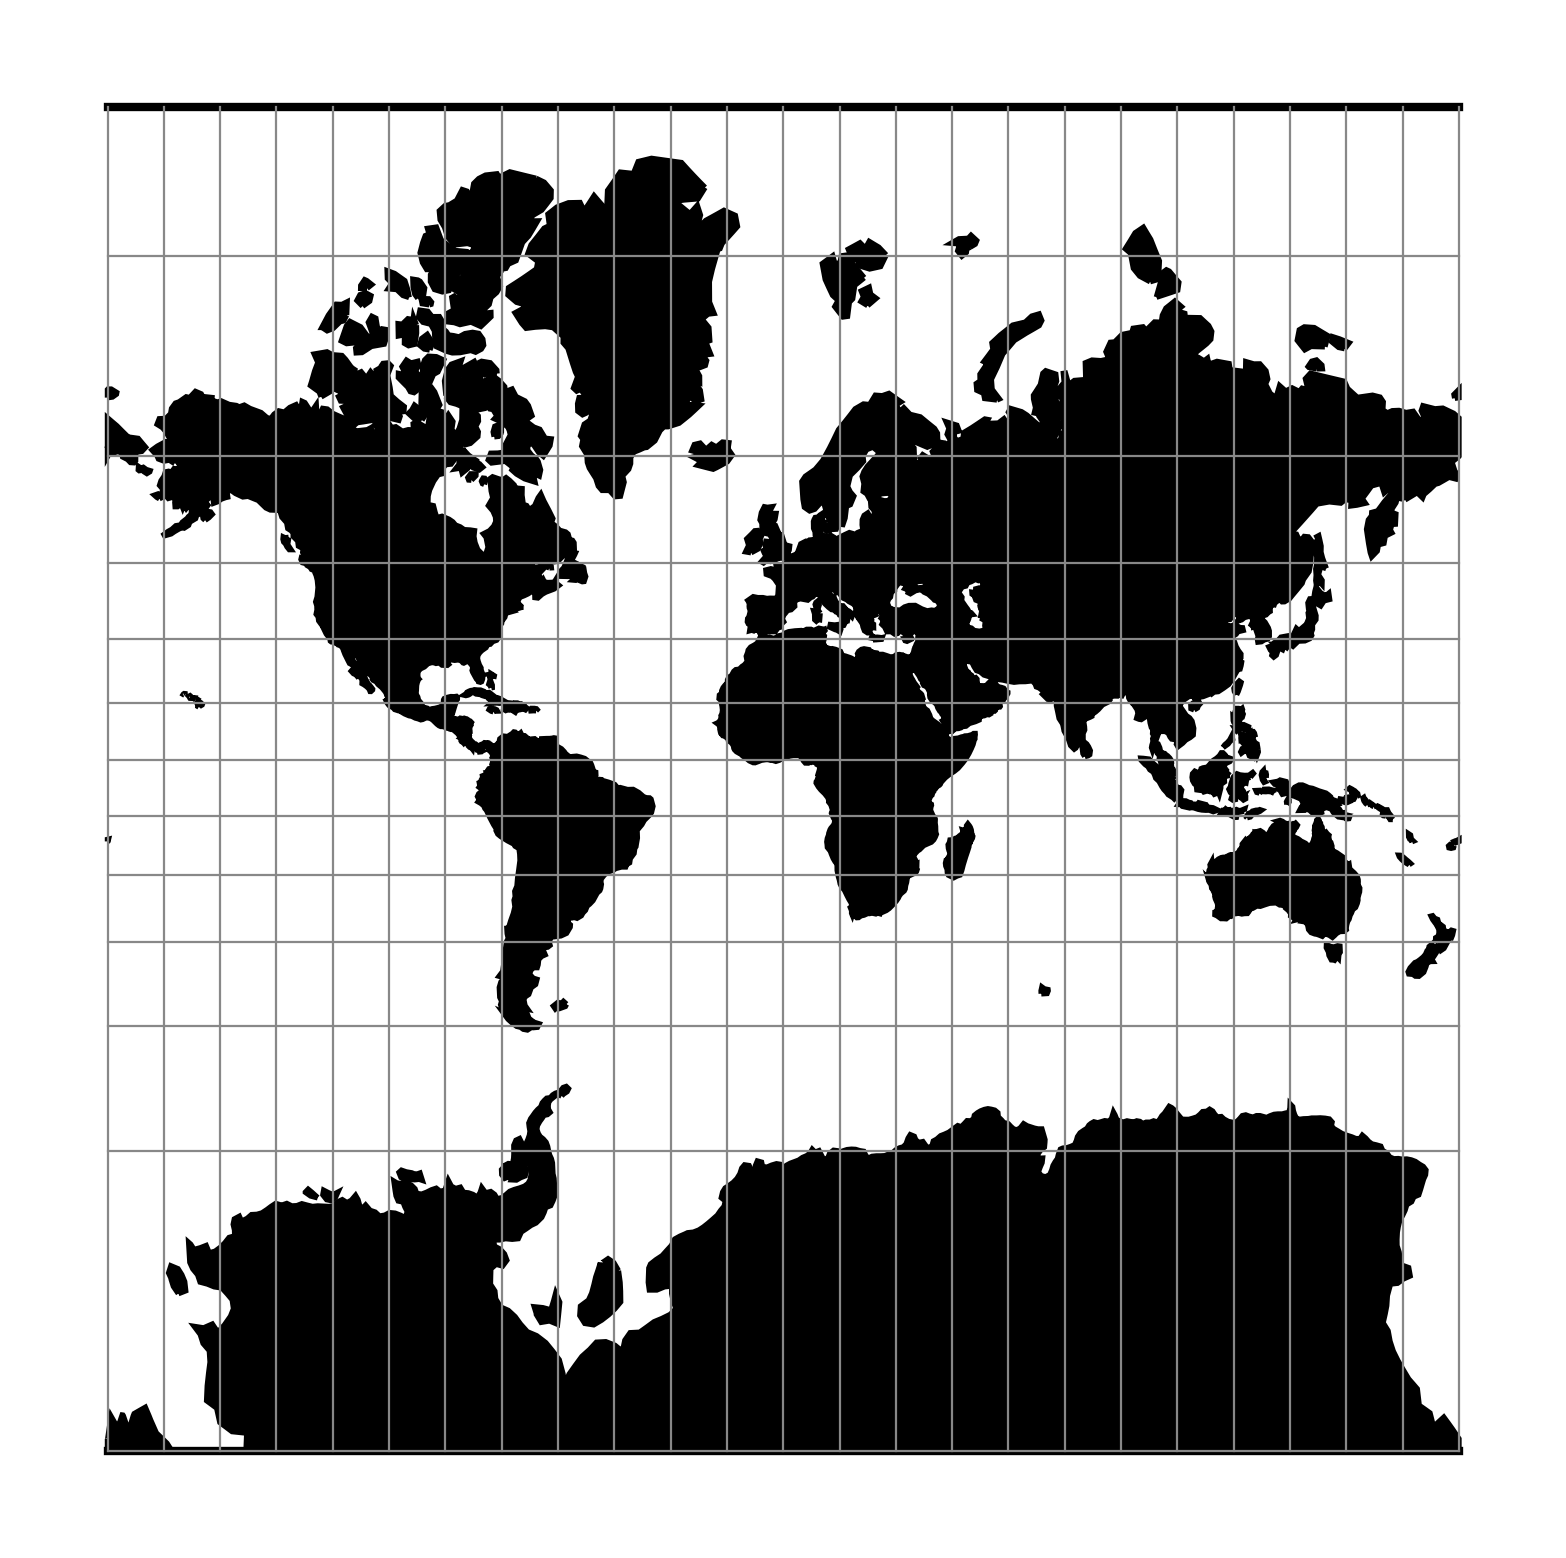
\includegraphics[width=0.5\linewidth]{figures/chapter-7/merc.png}
    \caption{Mercator projection (Source: \cite{PROJ_SITE})}
    \label{fig:mercator-projection}
\end{figure}

This "Proj.4" string transforms the EPSG: 4326 latitude and longitude coordinate pairs to the Mercator projected coordinates.

The advantages of using the "Proj.4" strings for the transformation are as follows:
"Proj.4" format strings are human-friendly and readable. The separation of the arguments for the transformation makes them understandable.
The "Proj.4" format allows us to change the transformation's parameters. Compared to the EPSG codes, which have fixed parameters regardless of whether we consider the projected or geodetic coordinate reference systems, the " Proj. 4 " format allows you to change the transformation's parameters.
Some of the parameters +datum or +R give precise control over the transformation. These parameters are about the ellipsoid used for the transformation.

A complete list of all the shared arguments is in the table below, as some of the projections can have different arguments. Cartographers and geographers can better interpret the arguments.
@TODO: Adds references to these links [usman]
"https://loc.gov/preservation/digital/formats/fdd/fdd000548.shtml"
"Reference: https://mapscaping.com/a-guide-to-wkt-in-gis/"
\subsection{pyproj}
pyproj is a Python package that is an interface to Proj software. The package provides programming interfaces for using the "Proj.4" strings. Not only to handle the "Proj.4"  CRS format and the newer version, "Proj.5". The "Proj.4" is commonly used for projected reference systems in most GIS systems. The package can handle the EPSG-coded format for CRS as well. The main interface used in the preprocessing pipeline is the "Transformer" class, which takes the argument of the base coordinate reference system and the target projected reference system "Proj.4" string.

\section{Data transformation to projection}
Converting the geographic coordinate reference system is possible solely if the base reference system is provided. Direct conversion from one projected reference system to another is not possible. As mentioned in the chapter introduction, the ultimate goal of the preprocessing pipeline is to generate projected raster data. When the pipeline finishes processing, it generates a raster as the data is in the projected reference system.
It is worth mentioning that the conversion from one projected reference system to another involves a series of transformations.

The series of transformations are as follows:
\begin{itemize}
    \item The pairs of coordinates are in a projected reference system. The projected reference system coordinates will be first transformed to the geographic CRS coordinates.
    \item After the first step, the geographic CRS coordinates are transformed into the desired projected reference system.
\end{itemize}
\begin{figure}[h]
    \centering
    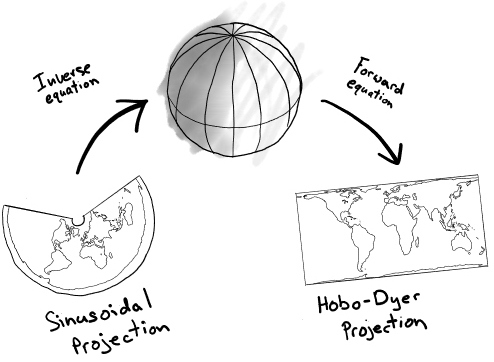
\includegraphics[width=0.5\linewidth]{figures/chapter-7/d_reprojection_example.jpg}
    \caption{transformation between projected reference systems (Source \cite{PROJ_IMAGES})}
    \label{fig:transformation-between-projected-reference-systems}
\end{figure}



Firstly, a CRS is specified for the coordinates that must go through the transformation into a projected reference system. After that, a conversion of the coordinates to the projected reference system is possible. This distinction was necessary because a CRS or a PRS are simply float numbers. The range of the latitudes and longitudes for CRS in ESPG:4326 is from -90 to -90 and 0 to 360, respectively. This base CRS ensures that data for conversion to the projected reference system does not violate the ranges. Otherwise, the underlying PROJ software throws an error regarding the values of the latitudes and longitudes are out of range. The actual value range of the longitudes is from -180 to 180, but PROJ allows the ranges above for the longitudes by radial calculations.\url{https://pygis.io/_images/d_reprojection_example.jpg}

The pyproj package's Transformer class is used to transform the coordinates. The class provides a function "from\_proj" to initialize the Transformer object for performing the transformations. The parameters for the Transformer class are the base CRS and the "Proj.4" string. The base CRS is in the EPSG code, which is 4326, equivalent to the "Proj.4" string "+proj=latlon." This Transformer object is used to create a mapping with the geographical data.

The original data is in a grid shape. The geospatial data chapter explains this property of the data. The conversion happens on a mapping of each latitude and longitude pair. Each pair of coordinates goes through the transformation (via the Transformer object) to the respective projected reference system mentioned in the pipeline settings. This mapping also associates any geographic data with the pairs of transformed coordinates. Thus, it completes the transformation of the latitude and longitude pairs to the projected coordinate reference system and creates the association with the geographical data.


\section{Data Interpolation }
It is common practice to analyze geospatial data by generating data rasters, which can be of any dimension. In our case, the resolution or dimension of the data is 240 by 240. The chapter concerning data explains the dimensions of the original data. If we place the data in the 240 by 240 grid, that data grid would be sparse. A 240 by 240 grid means 57600 data points. The problem then becomes of the form of multivariate regression. Different regression algorithms are used to generate the rasters to overcome the issue of the data's sparsity.The preprocessing pipeline offers two types of regression algorithms.

\begin{itemize}
    \item K-nearest neighbor regression
    \item Gaussian process regression
\end{itemize}
For the experimentation, K-nearest neighbor regression is trained on the projected coordinates and the geographical data. K-nearest neighbors regression is a method utilized in statistical analysis for predicting continuous numerical values. The advantage of KNN regression is that it processes the data memory efficiently.

The previous section explains the data transformation. The transformation function returns a mapping of the projected coordinates with the geographical data. This mapping is then used for the training of the k-nearest neighbor regressor. This regressor is trained by the hyperparameter of k=10. The machine learning library sklearn is used for the regression algorithms. This step returns a trained regressor, which is used in the further steps for generating the data raster.
\begin{figure}[h]
    \centering
    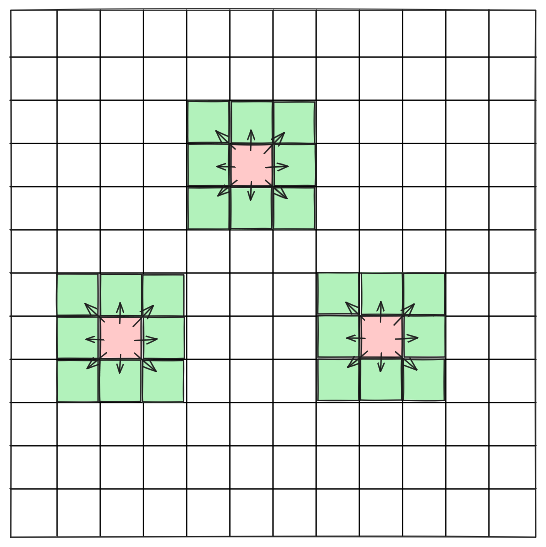
\includegraphics[width=0.5\linewidth]{figures/chapter-7/raster_interpolation.png}
    \caption{K-nearest neighbor learning}
    \label{fig:knn-learning}
\end{figure}

\section{Raster Data Generation}

Generating the data raster according to the resolution entails a series of steps that utilize the Numpy spline function. The minimum and the maximum of the projected coordinates are calculated. By leveraging this information, it becomes possible to accurately generate equi-spaced projected coordinates that align with the desired resolution of the raster.
The spline function considers the projected coordinates and utilizes them to generate equispaced coordinates. It achieves this by considering the raster's resolution and ensuring that the generated coordinates are distributed in a manner that aligns with the given resolution.
Following this, the trained regressor, specifically the K-nearest neighbor in our case, is utilized to predict the values for the geographical data that will populate the raster. In our scenario, a raster of 240 by 240 was employed. This concludes the process of creating a singular raster.

\subsection{Generation Settings}
This section explains the main arguments required to generate the raster data. The first argument of 'projection' takes in an enum value associated with the Proj.4 strings for different projections. The 'regressor\_type' takes the value of which regressor is used. The resolution argument plays an important role in defining the resolution of the raster and the input shape of the convolutional neural network used in the experimentation.
\begin{itemize}
    \item \textbf{Projection}: This argument provides the projection string according to the \textbf{Proj.4} format.
    \item  \textbf{Regression Type}: This argument takes the regerssion type for raster data generation, for the experimentation K-nearest neighbor regression was used for dataset generation.
    \item \textbf{Resolution}: The resolution is to define the height and the width of the raster, as raster data is in a grided form.
\end{itemize}

% \begin{lstlisting}[language=Python, caption=Pipeline raster data settings]
% class PipelineSettings(BaseModel):
%     projection: Projections
%     regressor_type: RegressorEnum
%     resolution: int 
% \end{lstlisting}

\subsection{Generation Step}
\begin{algorithm}
    \caption{Preprocessing steps}
    \label{}
    \begin{algorithmic}[1]
        \FOR{ each data point in the list given to the preprocessing pipeline}
        \STATE Extracts the Latitudes and Longitudes for each data point
        \STATE Creates a Transformer object for the coordinates transformation
        \STATE Generates a mapping of the geographical data with the projected coordinates
        \STATE Trains a regression model from mapping with projected coordinates and geographical data
        \STATE Extracts the minimum and maximum values of the projected coordinates
        \STATE Generates the equispaced arrays from the minimum and maximum values of the coordinates using NumPy's spline
        \STATE Predicts the values to fill the raster using the mappings of the newly generated equispaced coordinates  using the trained regression model

        \ENDFOR
        \STATE Returns the data raster list
    \end{algorithmic}
\end{algorithm}